\chapter{Learning the parameters of a state-space model}
\label{chap:inference}

This chapter describes the state-space model (SSM) formulation we are working with. In \autoref{sec:ssm-definition}, we state our assumptions about the individual probability distributions. Then in \autoref{sec:parameter-inference}, we calculate the posterior distribution of the parameters of interest, and show that straightforward inference is not possible. Further on, we derive a sampler to approximate this distribution. By itself, this sampler is unusable, as it requires the evaluation of the model likelihood. To circumvent this, we introduce the particle filter in \autoref{sec:particle-filter}. This section gives the definition and some of the properties of the filter. Later in \autoref{sec:particle-filter-estimate} we show how to use the particle filter to estimate the likelihood, and argue that it does not affect the asymptotic properties of the sampler.

Most of this chapter is based on \cite{andrieu} and \cite{schoen}.



\section{State-Space Model definition} \label{sec:ssm-definition}
The state-space model, often also called the hidden Markov model (HMM) assumes a sequence of latent states $\left\{\bx_t\right\}_{t=0}^\infty \subseteq \R^{d_x}$ following a Markov chain, and a sequence of observed variables $\left\{\by_t\right\}_{t=1}^\infty \subseteq \R^{d_y}$. All involved distributions are parameterized by an unknown static parameter $\btheta \in \Theta \subset \R^d$.

For a fixed time $T \geq 1$, we use the shorthands $\bx_{0:T} = \left\{\bx_t\right\}_{t=0}^T$ and $\by_{1:T} = \left\{\by_t\right\}_{t=1}^T$.

The HMM formulation means that the joint distribution of $\bx_{0:T}$ and $\by_{1:T}$ factorizes, for any $T \geq 1$, into
\begin{equation}\label{eq:factorization}
p(\bx_{0:T}, \by_{1:T} \mid \btheta) = \sprior(\bx_0 \mid \btheta) \prod_{t = 1}^{T} \trans_t(\bx_t \mid \bx_{t-1}, \btheta) \obs_t(\by_t \mid \bx_t, \btheta),
\end{equation}
where $\sprior$ is the prior distribution over the initial state, $\trans_t$ is the transition distribution at time $t$ and $\obs_t$ is the observation model at time $t$.

The factorization \eqref{eq:factorization} can be written more clearly as
\begin{align*}
\bx_0 \mid \btheta & \sim \sprior(\cdot \mid \btheta), \\
\bx_t \mid \bx_{t-1}, \btheta & \sim \trans_t(\cdot \mid \bx_{t-1}, \btheta), \quad t = 1, \ldots, T, \\
\by_t \mid \bx_t, \btheta & \sim \obs_t(\cdot \mid \bx_t, \btheta), \quad t = 1, \ldots, T.
\end{align*}

Finally, in accordance with the Bayesian approach \citep{bayes}, we introduce a prior distribution $\pprior$ over the unknown parameters $\btheta$ quantifying our knowledge about $\btheta$ before observing any data. This allows us to state the full joint distribution
\begin{equation}\label{eq:full-joint}
p(\bx_{0:T}, \by_{1:T}, \btheta) = p(\bx_{0:T}, \by_{1:T} \mid \btheta) \pprior(\btheta).
\end{equation}
The corresponding graphical model is depicted in \autoref{fig:graphical-model}.
\begin{figure}[ht]
    \centering
    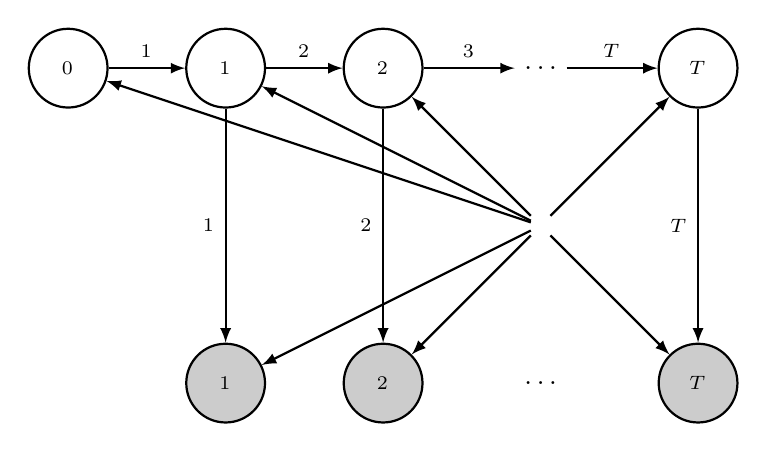
\begin{tikzpicture}
    % Style
    \tikzstyle{main}=[circle, minimum size = 10mm, thick, draw =black!80, node distance = 16mm]
    \tikzstyle{connect}=[-latex, thick]
    
    % Nodes X
    \node[main,shape=circle,draw=black](X0) at (1,4) {$\bx_0$};
    \node[main,shape=circle,draw=black](X1) at (3,4) {$\bx_1$};
    \node[main,shape=circle,draw=black](X2) at (5,4) {$\bx_2$};
    \node[](Xdots) at (7,4) {$\ldots$};
    \node[main,shape=circle,draw=black](XT) at (9,4) {$\bx_T$};
    
    % Node theta
    \node[](theta) at (7,2) {$\btheta$};
    
    % Nodes Y
    \node[main,shape=circle,draw=black,fill=black!20](Y1) at (3,0) {$\by_1$};
    \node[main,shape=circle,draw=black,fill=black!20](Y2) at (5,0) {$\by_2$};
    \node[](Ydots) at (7,0) {$\ldots$};
    \node[main,shape=circle,draw=black,fill=black!20](YT) at (9,0) {$\by_T$};

    % Edges XX
    \path [->] (X0) edge[connect] node[left] [above] {$\trans_1$} (X1);
    \path [->] (X1) edge[connect] node[left] [above] {$\trans_2$} (X2);
    \path [->] (X2) edge[connect] node[left] [above] {$\trans_3$} (Xdots);
    \path [->] (Xdots) edge[connect] node[left] [above] {$\trans_T$} (XT);
    
    % Edges XY
    \path [->] (X1) edge[connect] node[left] [left] {$\obs_1$} (Y1);
    \path [->] (X2) edge[connect] node[left] [left] {$\obs_2$} (Y2);
    \path [->] (XT) edge[connect] node[left] [left] {$\obs_T$} (YT);
    
    % Edges theta X
    \path [->] (theta) edge[connect] node[left] {} (X0);
    \path [->] (theta) edge[connect] node[left] {} (X1);
    \path [->] (theta) edge[connect] node[left] {} (X2);
    \path [->] (theta) edge[connect] node[left] {} (XT);
    
    % Edges theta Y
    \path [->] (theta) edge[connect] node[left] {} (Y1);
    \path [->] (theta) edge[connect] node[left] {} (Y2);
    \path [->] (theta) edge[connect] node[left] {} (YT);
    \end{tikzpicture}
    \caption{Graphical model describing the full joint distribution \eqref{eq:full-joint}. The shaded nodes denote the observed variables, white nodes represent the latent variables.}
    \label{fig:graphical-model}
\end{figure}



\section{Parameter inference} \label{sec:parameter-inference}
Given an observed sequence $\by_{1:T}$, Bayesian inference relies on the joint posterior density
\begin{equation}\label{eq:joint-posterior}
p(\btheta, \bx_{0:T} \mid \by_{1:T}) = \underbrace{p(\bx_{0:T} \mid \btheta, \by_{1:T})}_{\text{State inference}} \underbrace{p(\btheta \mid \by_{1:T})}_{\text{Parameter inference}}.
\end{equation}
Our primary interest is to perform inference about the static parameter $\btheta$. From \eqref{eq:joint-posterior}, it is clear that to infer about the hidden states $\bx_{0:T}$, one needs knowledge about $\btheta$, so even if the hidden states are of interest, inference about $\btheta$ is necessary. \autoref{sec:particle-filter-estimate} actually shows how to estimate $\bx_{0:T}$ as a by-product.


\paragraph{Bayesian inference}

To perform Bayesian inference about $\btheta$, we express the posterior of $\btheta$ by applying the Bayes theorem:
\begin{equation*}
p(\btheta \mid \by_{1:T}) = \frac{p(\by_{1:T} \mid \btheta) \pprior(\btheta)}{\int p(\by_{1:T} \mid \btheta) \pprior(\btheta) \dx{\btheta}}.
\end{equation*}

Evaluating the likelihood $p(\by_{1:T} \mid \btheta)$ requires marginalizing over $\bx_{0:T}$:
\begin{equation*}
p(\by_{1:T} \mid \btheta) = \int p(\bx_{0:T}, \by_{1:T} \mid \btheta) \dx{\bx_{0:T}},
\end{equation*}
where $p(\bx_{0:T}, \by_{1:T} \mid \btheta)$ is given in \eqref{eq:factorization}. Unless the SSM is linear and Gaussian, such $d_x(T+1)$-dimensional integral is intractable \citep{andrieu}.


\paragraph{Inference under tractable likelihood assumption}

For the time being, we proceed as if the likelihood was tractable. We derive a sampler for $\btheta$ and note which component cannot be evaluated due to the likelihood being present. \autoref{sec:particle-filter-estimate} then describes the necessary changes to allow circumventing the likelihood evaluation.

Often, the interest is not in the posterior $p(\btheta \mid \by_{1:T})$ itself, but on the expectation of some function $\phi$ w.r.t. this distribution, i.e. on
\begin{equation} \label{eq:posterior-integral}
\E_{p(\btheta \mid \by_{1:T})}[\phi(\btheta)] = \int \phi(\btheta) p(\btheta \mid \by_{1:T}) \dx{\btheta}.
\end{equation}
We use the Metropolis-Hastings algorithm \citep{metropolis, hastings} to obtain $M$ samples from $p(\btheta \mid \by_{1:T})$, denoted as $\btheta^{(m)},\ m = 1, \ldots, M$. The integral \eqref{eq:posterior-integral} is then approximated as the arithmetic mean
\begin{equation*}
\frac{1}{M} \sum_{m=1}^M \phi(\btheta^{(m)}).
\end{equation*}
An appealing property of the Metropolis-Hastings algorithm is that such arithmetic mean converges to \eqref{eq:posterior-integral} almost surely \citep{robert-casella}, i.e.
\begin{equation*}
\frac{1}{M} \sum_{m=1}^M \phi(\btheta^{(m)}) \xrightarrow{a.s} \int \phi(\btheta) p(\btheta \mid \by_{1:T}) \dx{\btheta},
\end{equation*}
where $\xrightarrow{a.s.}$ denotes almost sure convergence.

Finally, we note that if one is indeed interested in the distribution $p(\btheta \mid \by_{1:T})$ itself, it can be recovered by the empirical distribution
\begin{equation*}
\hat{p}(\btheta \mid \by_{1:T}) = \frac{1}{M} \sum_{m=1}^M \delta_{\btheta^{(m)}}(\btheta),
\end{equation*}
where $\delta$ denotes the Dirac distribution. This estimate can be additionally smoothed using kernel methods \citep{kernel-smoothing}.


\paragraph{Metropolis-Hastings algorithm}
The Metropolis-Hastings algorithm is described in \autoref{alg:metropolis-hastings}. Although well-known, it is included for comparison with the variant introduced in \autoref{sec:particle-filter-estimate}.

The target distribution is the parameter posterior $p(\btheta \mid \by_{1:T}) \propto p(\by_{1:T} \mid \btheta) \pprior(\btheta)$. In this case, it is not necessary to evaluate the normalizing constant, since it gets cancelled out.

The algorithm further requires a proposal distribution $\prop$. Similarly to the prior $\pprior$, it is problem-dependent, and must be selected carefully.

\begin{algorithm}[ht]
    \caption{Metropolis-Hastings}
    \label{alg:metropolis-hastings}
    \begin{algorithmic}[1]
        \Input $\text{Number of samples } M,\ \left\{\by_1, \ldots, \by_T\right\}$
        
        \State $\text{Initialize } \btheta^{(0)}.$
        
        \For{$m = 1\ \mathbf{to}\ M$}
            \State $\text{Sample } \btheta^\prime \sim \prop(\cdot \mid \btheta^{(m-1)}).$
            \State $\text{Calculate the aceptance probability } $ \begin{equation} \label{eq:acceptance-probability}
            \alpha = \min \left\{1, \frac{p(\by_{1:T} \mid \btheta^\prime) \pprior(\btheta^\prime)}{p(\by_{1:T} \mid \btheta^{(m-1)}) \pprior(\btheta^{(m-1)})} \frac{\prop(\btheta^{(m-1)} \mid \btheta^\prime)}{\prop(\btheta^\prime \mid \btheta^{(m-1)})} \right\}.
            \end{equation}
            \State $\text{Sample } u \sim \mathcal{U}(0,1).$
            \If {$u \leq \alpha$}
                \State $\btheta^{(m)} \gets \btheta^\prime$ \Comment{With probability $\alpha$, accept the proposed sample.}
            \Else
                \State $\btheta^{(m)} \gets \btheta^{(m-1)}$ \Comment{With probability $1 - \alpha$, reject the proposed sample.}
            \EndIf
        \EndFor
        
        \Output $\left\{ \btheta^{(1)}, \ldots, \btheta^{(M)} \right\}$
    \end{algorithmic}
\end{algorithm}

We see that the acceptance probability \eqref{eq:acceptance-probability} cannot be calculated, as it depends on the intractable likelihood $p(\by_{1:T} \mid \btheta)$. In \autoref{sec:particle-filter-estimate}, we give a modified variant of the Metropolis-Hastings algorithm, where the likelihood is approximated using the particle filter. The derivation of this filter is the content of the next section.



\section{The particle filter} \label{sec:particle-filter}
The particle filter \citep{particle-filter} is a method for approximating the filtering distribution $p(\bx_t \mid \by_{1:t})$ using a finite number of samples called particles. The algorithm is also known as sequential Monte Carlo or sequential importance sampling. The latter name sheds some light on how the method works, and it is exactly through importance sampling that the particle filter is derived.

\paragraph{Importance sampling}
Here we briefly review the basic idea behind importance sampling. For a more thorough treatment, the reader is referred to \cite{information-theory} or \cite{robert-casella}.

Consider a situation where the expectation of some function $\phi$ w.r.t. the distribution with density $p$,
\begin{equation} \label{eq:is-expectation}
\Phi \coloneqq \E_{p}[\phi(\bm{X})] = \int \phi(\bm{x}) p(\bm{x}) \dx{\bm{x}},
\end{equation}
is of interest. Assume that the integral is analytically intractable, and that one cannot generate samples from $p$ to approximate this expectation. Assume further that the density $p$ can be evaluated, at least up to a multiplicative constant, i.e. that it takes the form
\begin{equation*}
p(\bm{x}) = \frac{p^*(\bm{x})}{Z},
\end{equation*}
where $Z$ is an unknown normalizing constant, and $p^*$ can be evaluated. Such situation frequently arises in Bayesian statistics, where a posterior distribution of interest $p(\btheta \mid \bm{x}) = \frac{p(\bm{x} \mid \btheta) p(\btheta)}{\int p(\bm{x} \mid \btheta) p(\btheta) \dx{\btheta}}$ is given in terms of the Bayes theorem. The normalizing constant in the denominator is often unavailable in analytic form. However, the numerator can be evaluated.

Next, we introduce a (typically simpler) distribution with probability density $q(\bm{x}) = \frac{q^*(\bm{x})}{Z_Q}$ such that
\begin{enumerate}
    \item One can sample from $q$;
    \item One can evaluate $q^*$;
    \item $p(\bm{x}) > 0$ implies $q(\bm{x}) > 0$.
\end{enumerate}
The expectation \eqref{eq:is-expectation} can then be written as
\begin{equation*}
\Phi = \int \phi(\bm{x}) \frac{q(\bm{x})}{q(\bm{x})} p(\bm{x}) \dx{\bm{x}} = \int \phi(\bm{x}) \underbrace{\frac{p(\bm{x})}{q(\bm{x})}}_{w^*(\bm{x})} q(\bm{x}) \dx{\bm{x}} = \E_{q}[\phi(\bm{X}) w^*(\bm{X})],
\end{equation*}
where $w^*(\bm{x})$ are called the importance weights. By defining $w(\bm{x}) = \frac{p^*(\bm{x})}{q^*(\bm{x})}$, $\Phi$ can be approximated by
\begin{equation*}
\Phi \approx \widehat{\Phi} \coloneqq \frac{\sum_{i=1}^N \phi(\bm{x}^{(i)}) w(\bm{x}^{(i)})}{\sum_{i=1}^Nw(\bm{x}^{(i)})}, \quad \bm{x}^{(1)}, \ldots, \bm{x}^{(N)} \stackrel{iid}{\sim} q.
\end{equation*}
We note that by using $w$ instead of $w^*$ and normalizing by the weights sum instead of the sample size $N$, we bypass the evaluation of $Z$ and $Z_Q$, since they cancel out. The importance weights here account for correcting the discrepancy between the distribution $q$ and the true distribution $p$.

The estimator $\widehat{\Phi}$ converges to the true expectation $\Phi$ as $N \to \infty$. However, it is not necessarily unbiased \citep{information-theory}.


\paragraph{Sequential importance sampling (SIS)}
The SIS algorithm uses a weighted set of particles $\left\{\left(\bm{x}_t^{(i)}, w_t^{(i)} \right) : i = 1, \ldots, N \right\}$, to represent the filtering distribution $p(\bm{x}_t \mid \by_{1:t})$. To simplify notation, we write $w_t^{(i)}$ instead of $w_t(\bm{x}^{(i)})$ from now on. The empirical approximation to $p(\bm{x}_t \mid \by_{1:t})$ is then
\begin{equation*}
\hat{p}(\bm{x}_t \mid \by_{1:t}) = \frac{\sum_{i=1}^N w_t^{(i)} \delta_{\bm{x}_t^{(i)}}(\bm{x}_t)}{\sum_{i=1}^N w_t^{(i)}}.
\end{equation*}

As the name suggests, the algorithm involves a sequential application of the importance sampling procedure with increasing time $t$.

Returning to the SSM \eqref{sec:ssm-definition}, we consider the posterior distribution of a sequence of states $\bx_{0:t}$ given a sequence of observations $\by_{1:t}$. By application of the Bayes theorem, we obtain the following recursive formula:
\begin{equation*}
\begin{split}
p(\bx_{0:t} \mid \by_{1:t}) & \propto p(\by_t \mid \bx_{0:t}, \by_{1:t-1}) p(\bx_{0:t} \mid \by_{1:t-1}) \\
&= \obs_t(\by_t \mid \bx_t) p(\bx_t \mid \bx_{0:t-1}, \by_{1:t-1}) p(\bx_{0:t-1} \mid \by_{1:t-1}) \\
&= \obs_t(\by_t \mid \bx_t) \trans_t(\bx_t \mid \bx_{t-1}) p(\bx_{0:t-1} \mid \by_{1:t-1}),
\end{split}
\end{equation*}
where the equalities follow from the hidden Markov model independence assumptions.

\paragraph{Resampling}

\paragraph{The particle filter}



\section{Using the particle filter to estimate the likelihood} \label{sec:particle-filter-estimate}